%!TEX encoding = UTF-8 Unicode

%----------------------------------------------------------------------------------------
%	CHAPTER 2
%	Translator: InSight
%----------------------------------------------------------------------------------------

\chapterimage{chapter_head_1.pdf} % Chapter heading image

\makeatletter 
\newcommand\figcaption{\def\@captype{figure}\caption} 
\newcommand\tabcaption{\def\@captype{table}\caption} 
\makeatother

\chapter[狭义相对论]{Special Relativity 狭义相对论}
\label{chap2} 
著名的迈克尔逊-莫雷(Michelson-Morley)实验告诉我们,光在任何参考系中都具有相同的速度\mpar{我们日常生活中所观测到的物体的速度取决于选定的参考系。如果一个观者站在火车站上,测得的火车速度为$50 \frac{km}{h} $,另一个观者以$15\frac{km}{h} $ 的速度与火车一同运动,那么测得的火车速度就应是$35 \frac{km}{h}$。与此不同的是,光始终以$1.08 \times 10^9 \frac{km}{h}$运动,不论你如何相对于光运动。}。Albert Einstein第一个意识到这个结果所蕴含的深刻意义,在这一不寻常的自然真理的基础之上,他建立了狭义相对论。从光速不变原理出发,Einstein预言了许多有趣而又悖于常理的现象,这些现象最后都被证实是正确的。我们将看到这个原理是多么的强大,但是先让我们澄清有关狭义相对论的一些事实。狭义相对论的两个基本假设是
\begin{itemize}
	\item {\bf{相对性原理:}} 在任意惯性系中的物理规律均相同,例如两个相对速度恒定的惯性参考系。
	\item {\bf{光速不变原理:}} 在任意惯性系中的光速均为常数$c$。
\end{itemize}
除此之外,我们还假设物理时空均匀且具有各向同性。这意味着不论我们在哪儿(均匀),不论朝着什么方向(各向同性)做实验,物理规律都是一样的。举个例子,两个物理学家,一个在纽约,一个在东京,做完全一样的两个实验,他们会得到相同
\mpar{这当然要考虑到某些参数的影响,例如重力加速度。}  的物理规律,同样的,就算是在火星上的物理学家也会得到同样的物理规律。

%翻译欠佳,主语应该换换
一旦物理规律在数学上清晰地表达出来,那么,对于遵从该规律的物理实验而言,不管你是今天做,明天做,或是换个角度来看实验,它所蕴含的物理规律都应是不变的。此外,狭义相对论的第一条假设告诉我们,在匀速运动的马车上,或是在静止的实验室中,同一物理实验都会有相同的结果。以上论述均与实验相符。举个例子,如果你坐在匀速运动的汽车上,你没办法分辨出你是在运动还是静止。

一旦失去各向同性和均匀性,物理学将变得困难重重:我们从实验中得到的物理定律将仅仅在空间中的某一点对于确定的某一方向成立,这样的物理定律显然是毫无用处的。

唯一有些不直观的就是狭义相对论的第二条假设,毕竟它违背了我们的日常经验。虽然如此,至今为此所有的实验都表明这个假设是正确的。


\section[狭义相对论的不变量]{The Invariant of Special Relativity 狭义相对论的不变量}
\label{sec2.1}
在接下来的章节中,我们将使用狭义相对论的两个基本假设推导出Minkowski度规,有了它,我们就能计算两个物理事件的“距离”。所谓物理事件,是指在Minkowski 时空中的点,而整个狭义相对论都建立在Minkowski时空之上。{\it{任意两个不同惯性参考系之间的变换必须保证Minkowski度规不变,通过这一条件我们能到找两惯性系之间所有允许的变换。}}
%这也是我们如何能找到连接两惯性参考系之间所有允许的变换,例如那些光速为常数的参考系。(重新翻)}%所有连接两个不同惯性参考系的变换必须保证M度规不变,这也是我们如何找到
在本书剩下的部分我们将会用到这些关于变换的知识,来寻找在这些变换下都成立的方程。让我们从一个思想实验开始推出一些从基本假设出发得到的重要结论。

{\marginpar{
	\centering
	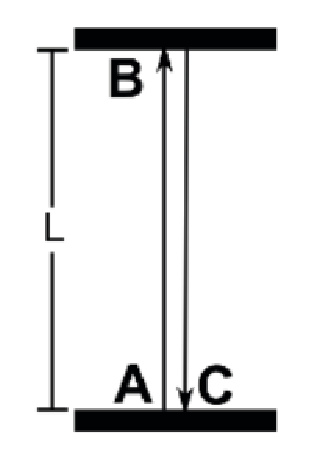
\includegraphics[scale=0.35]{fig2_1.eps}
	\figcaption{思想实验图示}
	\label{fig2.1}
}}

一个观者,站在他所处的坐标系的原点,向他的上方发出一个光脉冲,经过一段时间后被垂直镜面反射回原点。如图2.1所示

有3个重要的时刻:
\begin{itemize}
	\item {\bf{A:}}光从原点发出
	\item {\bf{B:}}光在镜面上反射
	\item {\bf{C:}}光回到原点
\end{itemize}
事件{\bf{AC}}之间的时间间隔为\mpar{对于匀速$v$来说,有$v=\frac{\Delta s}{\Delta t}$,$\Delta s$表示经过的距离,$\Delta t$代表所需时间,因此$\Delta t=\frac{\Delta s}{v}$}
\begin{equation}\label{eq2.1}
\Delta t=t_C-t_A=\frac{2L}{c}
\end{equation}
式中L表示原点与反射点之间的距离。

{\marginpar{
		\centering
		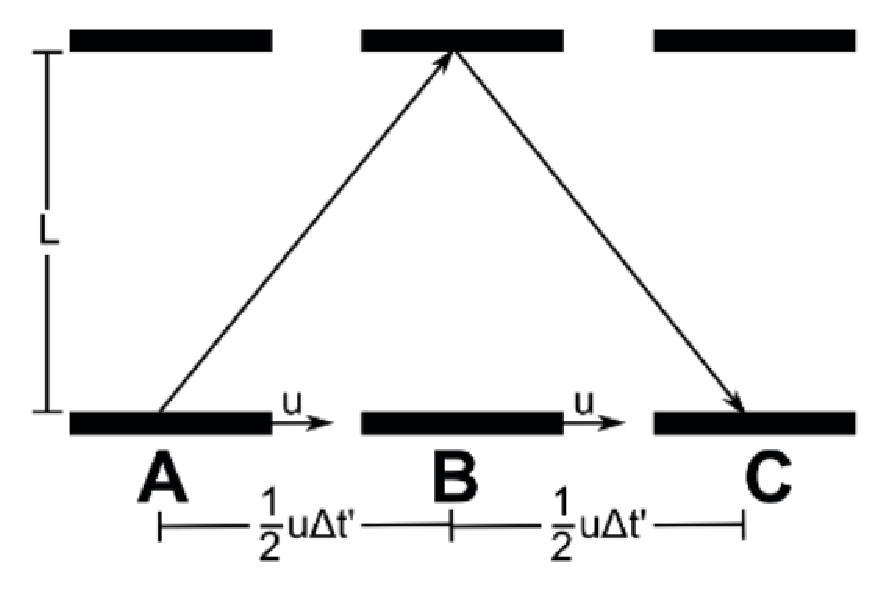
\includegraphics[scale=0.35]{fig2_2.eps}
		\figcaption{思想实验图示. 第二位移动观者向左移动, 因此第一位观者相对他向右移动}
		\label{fig2.2}
}}

接下来想象第二位观者,在$t_A$时刻处于他所在的坐标系的原点,并以恒定速度$u$相对于第一个观者\mpar{两个惯性参考系(即它们的相对速度恒定)之间物理量的变换称为{\bf{推动(Boost)}}变换, 后面我们会对此进行详述。}向左运动。为简便起见,我们假设第二个参考系的原点在$t_A$时刻与第一位观者的坐标系原点重合。第二位观者所见到的现象就与第一位不一样了。在他的参考系中,光脉冲的起点和终点并不在同一位置(见图2.2)。




我们用数学语言表示
\begin{equation}\label{eq2.2}
x'_A=0 \neq x'_C=u \Delta t' \qquad \rightarrow \qquad \Delta x' =u \Delta t'
\end{equation}
带撇物理量代表第二位观者所测量的量。对于第一位静止系的观者而言有
\begin{equation}
x_A=x_C \qquad \rightarrow \qquad \Delta x=0
\end{equation}
我们假定第二位观者运动沿x轴,因此
\begin{equation}
y'_A=y'_C \quad  \quad z'_A=z'_C \quad \rightarrow \quad \Delta y'=0 \quad  \quad \Delta z'=0
\end{equation}
那么同样也有
\begin{equation}
y_A=y_C \quad  \quad z_A=z_C \quad \rightarrow \quad \Delta y=0 \quad  \quad \Delta z=0
\end{equation}
接下来的问题是:{\bf{第二位观者所观测到的时间间隔是多少?}}因为我们假定了光速为常数,那么事件$AC$对于第二位观者而言将具有不同的间隔!时间间隔$\Delta t'=t'_C-t'_A$,等于光在第二位观者的参考系中走过的距离$l$除以光速$c$。
\begin{equation}\label{eq2.6}
\Delta t'=\frac{l}{c}
\end{equation}
{我们可以计算光传播的距离,利用古老的Pythagoras(毕达哥拉斯)定理(见图2.2)}
\begin{equation}
l=2 \sqrt{\left(\frac{1}{2} u \Delta t'\right)^2+L^2}
\end{equation}
利用式\ref{eq2.6}可以得到
\begin{equation}
c \Delta t' =2 \sqrt{\left(\frac{1}{2} u \Delta t'\right)^2+L^2}
\end{equation}
再利用式\ref{eq2.2}中的$\Delta x'=u\Delta t'$可得
\begin{displaymath}
c \Delta t' =
2 \sqrt{\left(\frac{1}{2} u \Delta t'\right)^2+L^2}
\end{displaymath}
\begin{displaymath}
\rightarrow
\left( c \Delta t' \right)^2 =
4 \left( \left(\frac{1}{2} u \Delta t'\right)^2+L^2 \right)
\end{displaymath}
\begin{equation}\label{eq2.9}
\rightarrow
\left( c \Delta t' \right)^2
-\left(\Delta x' \right)^2=
4 \left( \left(\frac{1}{2} u \Delta t'\right)^2+L^2 \right)
-\left(\Delta x' \right)^2 =4L^2
\end{equation}
现在回到式\ref{eq2.1},即$\Delta t =\frac{2L}{c}$,那么
\begin{equation}\label{eq2.10}
\left( c \Delta t' \right)^2
-\left(\Delta x' \right)^2
=4 L^2
=\left( c \Delta t \right)^2
=\left( \Delta t c \right)^2
-\underbrace{\left(\Delta x \right)^2}_{=0 \texttt{由式}2.3 \texttt{知}}
\end{equation}
终于,我们得到\mpar{{注意到我们在此处采用的是得到这个结果的最简方法,因为我们假定$t_A$时刻两坐标的原点重合。尽管如此,我们能够证明任意选择两惯性参考系的关系仍然能让结论成立,如果第二位观者的参考系运动方向任意,那就不再有$\Delta y'=0$和$\Delta z'=0$,但能够证明方程仍然是成立的,因为物理定律在任意惯性系中都是一样的,这也给了我们任意选择参考系来简化计算的自由,证明任意情况无非是再多花些功夫罢了。}}



\begin{equation}\label{eq2.11}
\left( c \Delta t' \right)^2
-\left(\Delta x' \right)^2
-\underbrace{\left(\Delta y' \right)^2}_{=0}
-\underbrace{\left(\Delta z' \right)^2}_{=0}
=
\left( c \Delta t \right)^2
-\underbrace{\left(\Delta x \right)^2}_{=0}
-\underbrace{\left(\Delta y \right)^2}_{=0}
-\underbrace{\left(\Delta z \right)^2}_{=0}
\end{equation}
考虑第三个观者,相对于第一个观者以不同的速度运动,用同样的推理可以得到
\begin{equation}\label{eq2.12}
\left( c \Delta t'' \right)^2
-\left(\Delta x'' \right)^2
-\left(\Delta y'' \right)^2
-\left(\Delta z'' \right)^2
=
\left( c \Delta t \right)^2
-\left(\Delta x \right)^2
-\left(\Delta y \right)^2
-\left(\Delta z \right)^2
\end{equation}
因此,我们得到了一些对于所有观者都相同的量:即二次式
\begin{equation}\label{eq2.13}
(\Delta s)^2
\equiv\left( c \Delta t \right)^2
-\left(\Delta x \right)^2
-\left(\Delta y \right)^2
-\left(\Delta z \right)^2
\end{equation}

此外,我们还能看出对于不同观者,$(\Delta x)^2+(\Delta y)^2+(\Delta z)^2$或者说$(c\Delta t)^2$是不同的。我们将在下一节讨论这一点所蕴含的物理意义。
